%!TEX root = main.tex
\vspace{-1em}
\section{Non-Linear Models}
\vspace{-0.5em}

In this section, we extend our framework to approximate arbitrary classification losses within arbitrarily small bias. 

\vspace{-0.5em}
\subsection{Quantizing Polynomials} 
\vspace{-0.5em}

Given a degree $d$ polynomial $P(x) = \sum_{i = 0}^{d} m_i z^i$, which
Our goal is to evaluate at $\vec{a}^\top \vec{x}$, while quantizing $\vec{a}$, so as to preserve the value of $P( \vec{a}^\top \vec{x})$ in expectation. 

We will use $d$ independent quantizations of $\vec{a}$, $Q_1(\vec{a}), Q_2(\vec{a}), \ldots, Q_d(\vec{a})$. 
Given these quantizations, our reconstruction of the polynomial at $( \vec{a}^\top \vec{x})$ will be 
\vspace{-0.5em}
$$ Q(P) := \sum_{i = 0}^d m_i \prod_{j \leq i} Q_j(\vec{a})^\top \vec{x}.$$

\vspace{-1em}
The fact that this is an unbiased estimator of $P( \vec{a}^\top \vec{x} )$ follows from the independence of the quantizations. Using Lemma~\ref{lem:quant-facts} yields:

\begin{lemma}
\label{lem:poly-sec-moment-bound}
	$\E[ Q(P)^2 ] \leq \left(\sum_{i = 0}^d m_i r(s)^i (\vec{a}^\top \vec{x})^i\right)^2.$
\end{lemma} 




\vspace{-0.5em}
\subsection{Quantizing Smooth Classification Losses}
\vspace{-0.5em}

We now examine a standard classification setting, where samples $[(\vec{a}_i, b_i)]_i$ are drawn from a distribution $\mathcal{D}$. Given a smooth loss function $\ell: \R \rightarrow \R$,  we wish to find $\vec{x}$ which minimizes $\E_{\mathcal{D}} [ \ell( b \cdot \vec{a}^\top \vec{x}) ]$. The gradient of $\ell$ is given by 
$$ \nabla_\vec{x} (b \cdot \vec{a}^\top \vec{x}) = b \ell' (b \cdot \vec{a}^\top \vec{x}) \vec{a}.$$

Assume normalized samples, i.e. $\| \vec{a}_i \|_2 \leq 1, \forall i$, and that $\vec{x}$ is constrained such that $\| \vec{x} \|_2 \leq R$, for some real value $R > 0$. We we wish to approximate the gradient within some target accuracy $\epsilon$. 

To achieve this, fix a minimal-degree polynomial $P$ such that $|P(z) - \ell'(z)| \leq \epsilon, \forall z \leq R$. Assume this polynomial is known to both transmitter (sample source) and receiver (compute device). The protocol is as follows. 
\vspace{-0.5em}
\begin{itemize}
    \vspace{-0.5em}
	\item For a given sample $(\vec{a}_i, b_i)$ to be quantized, the source will transmit $b_i$, as well as $d + 1$ independent quantizations $Q_1, Q_2, \ldots, Q_{d + 1}$ of $\vec{a}_i$. 
    \vspace{-0.5em}
	\item The receiver computes $b \cdot Q(P) Q_{d + 1} ( \vec{a}_i )$ and uses it as the gradient.
\end{itemize}

\vspace{-0.5em}
It is easy to see that the bias in each step is bounded by $\epsilon$. 
We can extend Lemma~\ref{lem:poly-sec-moment-bound} to obtain a general guarantee on convergence. 

\begin{lemma}
	For any $\epsilon > 0$ and any convex classification loss function $\ell: \R \rightarrow \R$, there exists a polynomial degree $D(\epsilon, \ell)$ such that the polynomial approximation framework converges to within $\epsilon$ of OPT.  
\end{lemma}

\vspace{-0.5em}
\paragraph{Chebyshev Approximations} 
For \emph{logistic loss}, with sigmoid gradient, we notice that polynomial approximations have been well studied. In particular, we use the  Chebyshev polynomial approximation of~\cite{vlcek2012chebyshev}. 

\vspace{-0.5em}
\subsection{Quantizing Non-Smooth Classification Losses}
\vspace{-0.5em}

Our techniques further extend to convex loss functions with non-smooth gradients.  
For simplicity, in the following we focus on SVM, whose gradient (the step function), is discontinuous. 
This gradient is hard to approximate generally by polynomials; yet, the problem is approachable on intervals of the type  $[-R, R] \setminus [-\delta, \delta]$, for some small parameter $\delta > 0$~\cite{frostig2016principal, allen2016faster}; the latter reference provides the optimal approximation via Chebyshev polynomials, which we use in our experiments. 

The key challenge is that these results do any non-trivial guarantees for our setting, since gradients within the interval $[-\delta, \delta]$ can differ from the true gradient by $\Omega (1)$ in expectation. In particular, due to quantization, the gradient might be \emph{flipped}: 
its relative value with respect to $0$ changes, which corresponds to having the \emph{wrong} label for the current sample.\footnote{Training SVM with noisy labels has been previously considered previously, e.g.~\cite{Natarajan:2013:NIPS}, but in a setting where labels are corrupted uniformly at random. It is not hard to see that label corruptions are not uniform random in this case.}
We show two approaches for controlling the error resulting from these errors. 

The first is to just ignore such errors: under generative assumptions on the data, we can prove that quantization does not induce significant error. 
In particular, the error vanishes by taking more data points.
The second approach is more general: we use ideas from dimensionality reduction, specifically, low randomness Johnson-Lindenstrauss projections, to detect (with high probability) if our gradient could be flipped. If so, we refetch the full data points. 
This approach is always correct; however, it requires more communication.
Under the same generative assumptions, we show that the additional communication is \emph{sublinear} in the dimension.
Details are in the supplementary material.

\iffalse
Figure~\ref{fig:approximation} shows how close the Chebyshev polynomial aprroximations with different degrees are to those two kind of functions.

\begin{figure}[h]
\centering
    \begin{subfigure}[h]{.4\columnwidth}
    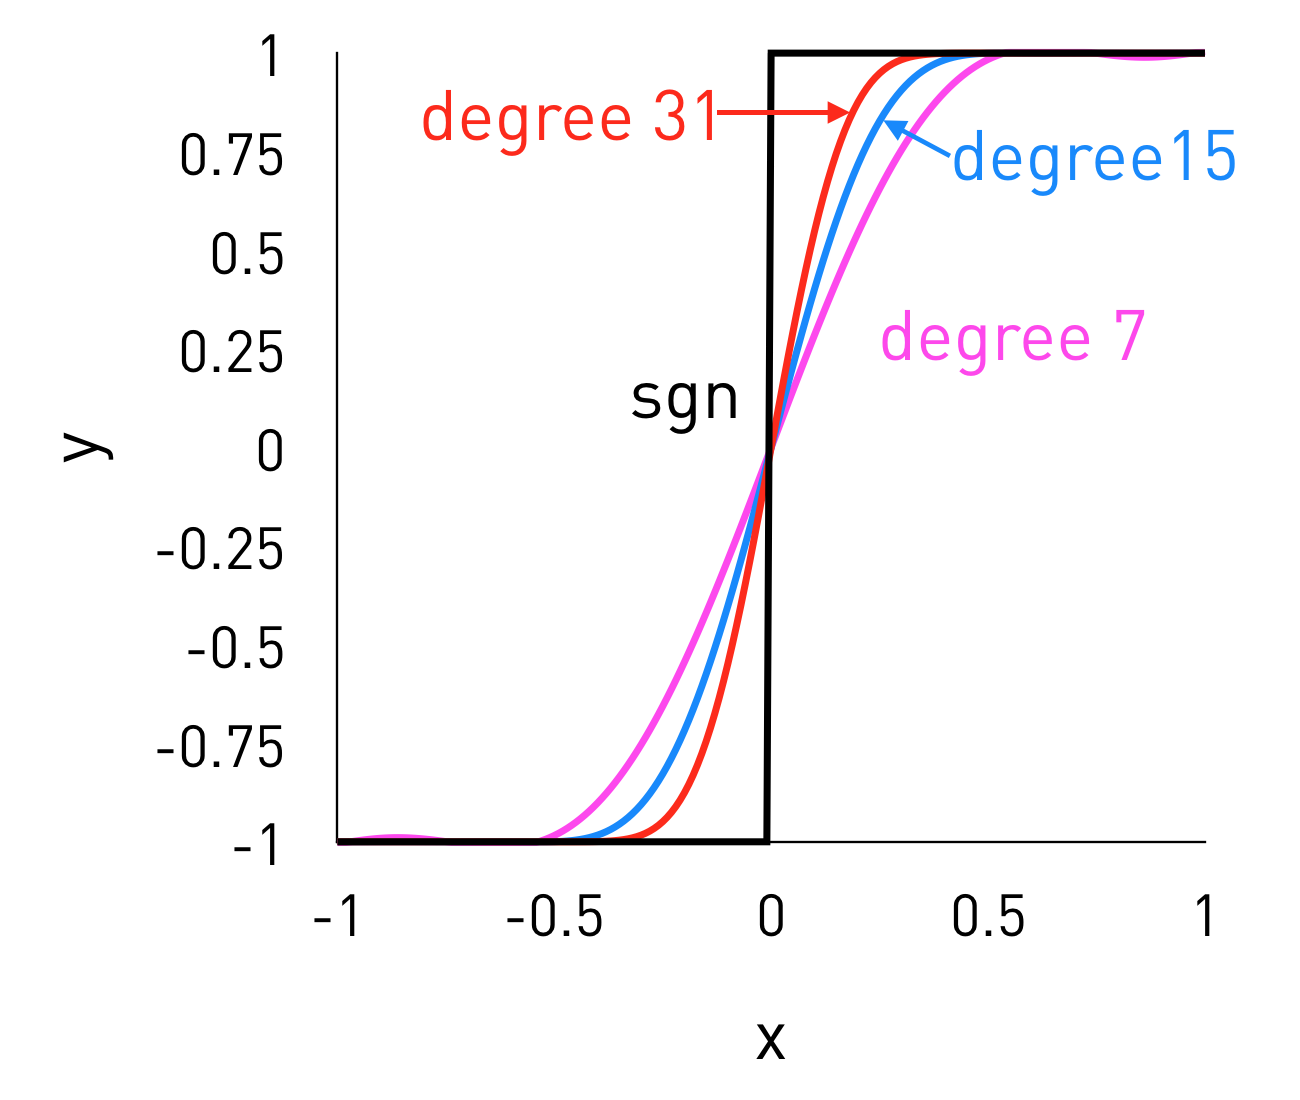
\includegraphics[width=\columnwidth]{micro-experiments/chebyshev_sgn} 
    \caption{sign function}
    \end{subfigure}
    \begin{subfigure}[h]{.4\columnwidth}
    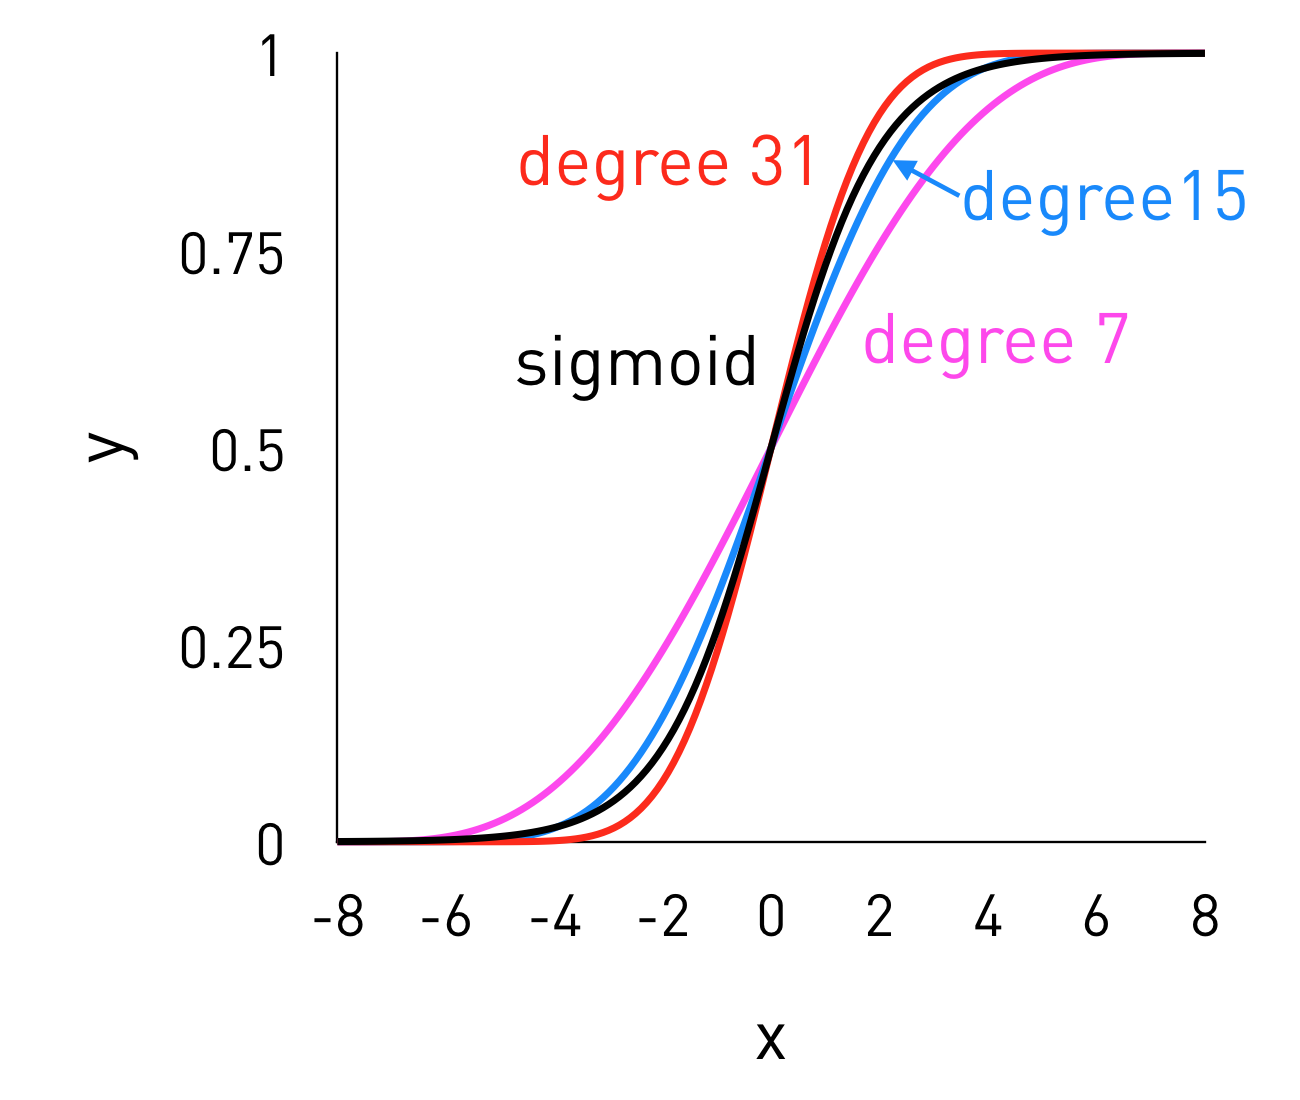
\includegraphics[width=\columnwidth]{micro-experiments/chebyshev_sigmoid} 
    \caption{sigmoid function}
    \end{subfigure}
\caption{Chebyshev approximation to gradient of hinge loss and logistic loss with different degrees}
\label{fig:approximation}
\end{figure} 
\fi

\vspace{-0.5em}
\paragraph{Practical Considerations} The above strategy introduces a precision-variance trade-off, since increasing the precision of approximation (higher polynomial degree) also increases the variance of the gradient. 
Fortunately, we can reduce the variance and increase the approximation quality by increasing the density of the quantization. 
In practice, a total of $8$ bits per sample in total to ensure convergence for both hinge and logistic loss. 

\vspace{-0.5em}
\paragraph*{The Refetching Heuristic}
The second theoretical approach inspires the following heuristic. 
Consider hinge loss, i.e.  $\sum_{k=1}^K \max(0, 1 - b_k \a_k^\top \x)$. 
We first transmit a single low-precision version of $\a_k$, and   
calculate upper and lower bounds on $b_k \a_k^\top \x$ at the receiver.
If the sign of $1-b_k \a_k^\top \x$ cannot change because of quantization, then we apply the approximate gradient. 
If the sign could change, then we {\em refetch} the data at full precision.
In practice, this works for 
8-bit while only refetching $<5\%$ of the data.

%\textcolor{red}{DAN: CAN WE SAY SOMETHING HERE ASSUMING LARGE MARGIN?}
%\textcolor{red}{Will look into this later.}

